\documentclass[]{article}
\usepackage{amssymb,amsmath}
\usepackage{ifxetex,ifluatex}
\ifxetex
  \usepackage{fontspec,xltxtra,xunicode}
  \defaultfontfeatures{Mapping=tex-text,Scale=MatchLowercase}
\else
  \ifluatex
    \usepackage{fontspec}
    \defaultfontfeatures{Mapping=tex-text,Scale=MatchLowercase}
  \else
    \usepackage[utf8]{inputenc}
  \fi
\fi
\usepackage{color}
\usepackage{fancyvrb}
\DefineShortVerb[commandchars=\\\{\}]{\|}
\DefineVerbatimEnvironment{Highlighting}{Verbatim}{commandchars=\\\{\}}
% Add ',fontsize=\small' for more characters per line
\newenvironment{Shaded}{}{}
\newcommand{\KeywordTok}[1]{\textcolor[rgb]{0.00,0.44,0.13}{\textbf{{#1}}}}
\newcommand{\DataTypeTok}[1]{\textcolor[rgb]{0.56,0.13,0.00}{{#1}}}
\newcommand{\DecValTok}[1]{\textcolor[rgb]{0.25,0.63,0.44}{{#1}}}
\newcommand{\BaseNTok}[1]{\textcolor[rgb]{0.25,0.63,0.44}{{#1}}}
\newcommand{\FloatTok}[1]{\textcolor[rgb]{0.25,0.63,0.44}{{#1}}}
\newcommand{\CharTok}[1]{\textcolor[rgb]{0.25,0.44,0.63}{{#1}}}
\newcommand{\StringTok}[1]{\textcolor[rgb]{0.25,0.44,0.63}{{#1}}}
\newcommand{\CommentTok}[1]{\textcolor[rgb]{0.38,0.63,0.69}{\textit{{#1}}}}
\newcommand{\OtherTok}[1]{\textcolor[rgb]{0.00,0.44,0.13}{{#1}}}
\newcommand{\AlertTok}[1]{\textcolor[rgb]{1.00,0.00,0.00}{\textbf{{#1}}}}
\newcommand{\FunctionTok}[1]{\textcolor[rgb]{0.02,0.16,0.49}{{#1}}}
\newcommand{\RegionMarkerTok}[1]{{#1}}
\newcommand{\ErrorTok}[1]{\textcolor[rgb]{1.00,0.00,0.00}{\textbf{{#1}}}}
\newcommand{\NormalTok}[1]{{#1}}
\usepackage{graphicx}
% We will generate all images so they have a width \maxwidth. This means
% that they will get their normal width if they fit onto the page, but
% are scaled down if they would overflow the margins.
\makeatletter
\def\maxwidth{\ifdim\Gin@nat@width>\linewidth\linewidth
\else\Gin@nat@width\fi}
\makeatother
\let\Oldincludegraphics\includegraphics
\renewcommand{\includegraphics}[1]{\Oldincludegraphics[width=\maxwidth]{#1}}
\ifxetex
  \usepackage[setpagesize=false, % page size defined by xetex
              unicode=false, % unicode breaks when used with xetex
              xetex,
              colorlinks=true,
              linkcolor=blue]{hyperref}
\else
  \usepackage[unicode=true,
              colorlinks=true,
              linkcolor=blue]{hyperref}
\fi
\hypersetup{breaklinks=true, pdfborder={0 0 0}}
\setlength{\parindent}{0pt}
\setlength{\parskip}{6pt plus 2pt minus 1pt}
\setlength{\emergencystretch}{3em}  % prevent overfull lines
\setcounter{secnumdepth}{0}


\begin{document}

\section{Ejercicios de programación I: Introducción}

\subsubsection{{[}IMSER 2013{]}}

\begin{center}\rule{3in}{0.4pt}\end{center}

\subsection{Archivos incluidos:}

El archivo con los ejercicios del práctico debe bajarse y descomprimirse
dentro de la carpeta del curso, creando la subcarpeta
\textbf{\texttt{rep-1}}. Usted deberá abrir el RStudio y seleccionar
dicha carpeta como su directorio de trabajo con \texttt{setwd} o en
RStudio la combinación \textbf{Ctrl + Shift + K}. En esta carpeta se
encuentran algunos archivos que usted deberá modificar:

\begin{itemize}
\item
  \textbf{\texttt{hipot.R}}
\item
  \textbf{\texttt{areaMax.R}}
\item
  \textbf{\texttt{dist.R}}
\item
  \textbf{\texttt{varianza.R}}
\item
  \textbf{\texttt{zenon.R}}
\item
  \textbf{\texttt{geom.R}}
\item
  \textbf{\texttt{shannon-1.R}}
\item
  \textbf{\texttt{shannon-2.R}}
\end{itemize}
Cada uno de estos archivos se corresponde con un ejercicio del
repartido. Se trata de archivos de texto plano (como un \texttt{.txt},
pero con extensión \texttt{.R}). En cada archivo se indica con presición
en dónde debe usted escribir su código (o modificar lo que ya está
escrito). Para que el sistema de corrección funcione bien, \textbf{no
cambie} el texto que se encuentra por fuera, incluyendo las que se usan
para indicar el inicio y el final del mismo. Nótese además que
\textbf{esto no impide} ampliar o reducir el espacio que usted tiene
para escribir, subiendo o bajando cualquiera de las ``líneas límite''
del archivo.

Adicionalmente los siguientes archivos son necesarios, pero \textbf{no
deben ser modificados} para que el método de calificación automático
funcione correctamente.

\begin{itemize}
\item
  \texttt{evaluar.R}
\item
  \texttt{datos}
\item
  \texttt{notas.csv}
\item
  \texttt{INSTRUCCIONES.pdf}
\end{itemize}
Nota: \emph{más recomendaciones importantes} se hacen en el documento
\href{http://eva.universidad.edu.uy/mod/resource/view.php?id=118422}{Dinámica
de los repartidos}.

\subsection{Mecanismo de corrección:}

Lo primero que debe hacer es cargar el archivo \texttt{evaluar.R} con la
función \texttt{source}:

\begin{Shaded}
\begin{Highlighting}[]
\KeywordTok{options}\NormalTok{(}\DataTypeTok{encoding =} \StringTok{"utf-8"}\NormalTok{)}
\KeywordTok{source}\NormalTok{(}\StringTok{"evaluar.R"}\NormalTok{)}
\end{Highlighting}
\end{Shaded}
Si usted ha ejecutado todos los pasos anteriores correctamente, la
siguiente frase debería verse en la consola:

\begin{verbatim}
Archivo de codigo fuente cargado correctamente
\end{verbatim}
En caso de que ocurra un error o se vea otro mensaje en la consola,
verifique que los archivos se descomprimieron correctamente y que usted
está trabajando en la carpeta correspondiente con el comando
\texttt{getwd()}.

Usted trabajará modificando los contenidos de dichos archivos con
RStudio (u otro programa de su preferencia) según las consignas que se
describen a continuación. Luego de terminar cada ejercicio y
\textbf{guardando el archivo} correspondiente en el disco duro, usted
podrá verificar rápidamente si su respuesta es correcta ejecutando el
comando:

\begin{Shaded}
\begin{Highlighting}[]
\KeywordTok{evaluar}\NormalTok{()}
\end{Highlighting}
\end{Shaded}
y además podrá en todo momento verificar su puntaje con la función
\texttt{verNotas()}. Una vez terminados los ejercicios del repartido,
usted deberá subir el archivo ''datos'' (sin extensión), incluido en la
carpeta ''rep-1'', a la
\href{http://eva.universidad.edu.uy/mod/assignment/view.php?id=93616}{sección
de entregas} de la portada del curso en la plataforma EVA.

\subsubsection{Código de Honor}

Si bien animamos a que trabaje en equipos y que haya un intercambio
fluido en los foros del curso, es fundamental que las respuestas a los
cuestionarios y ejercicios de programación sean fruto del trabajo
individual. En particular, consideramos necesario que no utilize el
código creado por sus compañeros, si no que debe programar sus propias
instrucciones, ya que de lo contrario supone un sabotaje a su propio
proceso de aprendizaje. Esto implica también evitar, en la medida de lo
posible, exponer el código propio a sus colegas. Como profesores estamos
comprometidos a dar nuestro mayor esfuerzo para dar las herramientas y
explicaciones adecuadas a fin de que pueda encontrar su propio camino
para resolver los ejercicios.

En casos de planteos de dudas a través del foro, en los que considere
que es imposible expresar un problema sin exponer su própio código,
entonces es aceptable hacerlo. De todas formas en estos casos es
preferible que envíe su código por correo electrónico directamente a un
profesor, explicando la problemática.

\begin{center}\rule{3in}{0.4pt}\end{center}

\subsection{1. Geometría}

Como sabrá probablemente, el filósofo (o grupo de filósofos) griego
Pitágoras es el supuesto autor del teorema homónimo, el cual sirve para
calcular la hipotenusa de un triángulo rectángulo. Este cálculo se
realiza con la fórmula $h^2 = a^2 + b^2$, en donde $h$ es la hipotenusa
y $a$ y $b$ los catetos.

\subsubsection{1.a Funciones simples}

Script: hipot.R

El siguiente código sirve para crear la función \texttt{hipot}, la cual
acepta como argumentos los anchos de los catetos y calcula el valor de
$h$ correspondientes:

\begin{Shaded}
\begin{Highlighting}[]
\NormalTok{hipot <- function(cat.ad, cat.op) \{}
    \NormalTok{out <- }\KeywordTok{sqrt}\NormalTok{(cat.ad^}\DecValTok{2} \NormalTok{+ cat.op^}\DecValTok{2}\NormalTok{)}
    \NormalTok{out}
\NormalTok{\}}
\end{Highlighting}
\end{Shaded}
Nótese que los objetos* \texttt{cat.ad} y \texttt{cat.op} son los
``argumentos'' de la función (y eso lo sabemos porque están dentro del
paréntesis que sigue a la función especial \texttt{function}). En las
líneas ``internas'' (i.e.: aquellas que están entre el \texttt{\{}
inicial y el \texttt{\}} final) de las funciones que haremos en este
repartido usaremos, por ahora, sólamente estos objetos para hacer todos
los cálculos requeridos.

(*: estrictamente no son objetos, en el sentido de objetos existentes en
nuestra sesión; de todas formas representan objetos que existen
temporalmente en el momento en que la función es evaluada. Veremos más
sobre este tema en la unidad 6)

Tomando este caso como ejemplo, complete el código del script
``hipot.R'' para hacer las funciones \texttt{area} y \texttt{co} tales
sean capaces de calcular el área de un triángulo y el cateto opuesto
respectivamente. Las entradas para la función \texttt{area}, es decir,
sus argumentos, serán los anchos de los catetos (tal como el la función
\texttt{hipot}, incluyendo el órden). Para el caso de \texttt{co} los
argumentos serán los anchos del cateto adyacente y de la hipotenusa,
\textbf{en ese orden}. Recuerde que para ejecutar este script debe usar
la función \texttt{source} de la siguiente manera:

\begin{Shaded}
\begin{Highlighting}[]
\KeywordTok{source}\NormalTok{(}\StringTok{"hipot.R"}\NormalTok{)}
\end{Highlighting}
\end{Shaded}
o usar los atajos de teclado de RStudio. Luego en la sesión de trabajo
aparecerán los distintos objetos definidos en el script (verifíquelo con
\texttt{ls()}), incluyendo a las funciones \texttt{area} y \texttt{co}.

Si sus funciones están correctas, usted debería obtener estos
resultados:

\begin{Shaded}
\begin{Highlighting}[]
\KeywordTok{area}\NormalTok{(}\DecValTok{3}\NormalTok{, }\DecValTok{4}\NormalTok{)}
\end{Highlighting}
\end{Shaded}
\begin{verbatim}
## [1] 6
\end{verbatim}
\begin{Shaded}
\begin{Highlighting}[]
\KeywordTok{co}\NormalTok{(}\DecValTok{3}\NormalTok{, }\DecValTok{5}\NormalTok{)}
\end{Highlighting}
\end{Shaded}
\begin{verbatim}
## [1] 4
\end{verbatim}
Nota: dado que para obtener el cateto se hace una resta, a cuyo
resultado se debe hallar la raíz cuadrada, considere que debe evitar
valores negativos. La forma más básica de evitarlo es encontrando el
valor absoluto, usando la función \texttt{abs}.

\subsubsection{1.b Área máxima}

Script: areaMax.R

En la lección 1.2 vimos cómo con un loop podemos ver fácilemnte todos
los valores posibles de salida de la función \texttt{prp}. Ahora
queremos hacer algo similar con la función \texttt{area}. Es decir, si
el cateto adyacente $x$ puede tomar cualquier valor tal que $0 < x < h$
(siendo $h$ la hipotenusa), entonces podemos buscar cuál es el área
máxima posible y para qué valor de $x$ se da. Obviamente este resultado
se puede encontrar analíticamente, pero para los propósitos del
ejercicio es útil calcularlo numéricamente.

Siguiendo el ejemplo de la lección 1.2 entonces el siguiente código
serviría para encontrar esa área (suponiendo que las funciones
\texttt{area} y \texttt{co} están correctamente definidas):

\begin{Shaded}
\begin{Highlighting}[]
\NormalTok{hip <- }\DecValTok{10}
\NormalTok{cat.ad <- }\KeywordTok{seq}\NormalTok{(}\FloatTok{0.001}\NormalTok{, hip - }\FloatTok{0.001}\NormalTok{, }\DataTypeTok{by =} \FloatTok{0.1}\NormalTok{)}
\NormalTok{for (i in }\DecValTok{1}\NormalTok{:}\KeywordTok{length}\NormalTok{(cat.ad)) \{}
    \NormalTok{cat.op <- }\KeywordTok{co}\NormalTok{(cat.ad[i], hip)}
    \KeywordTok{cat}\NormalTok{(}\StringTok{"ancho del cateto ad.:"}\NormalTok{, cat.ad[i], }\StringTok{"}\CharTok{\textbackslash{}n}\StringTok{"}\NormalTok{)}
    \KeywordTok{cat}\NormalTok{(}\StringTok{">> area:"}\NormalTok{, }\KeywordTok{area}\NormalTok{(cat.ad[i], cat.op), }\StringTok{"}\CharTok{\textbackslash{}n}\StringTok{"}\NormalTok{)}
\NormalTok{\}}
\end{Highlighting}
\end{Shaded}
Si usted ejecuta este código, podrá ver que el área máxima está cercana
a 25 y que el ancho del cateto adyacente correspondiente es
aproximadamente 7.1 (si ejecuta el script ``ejTriang.R'' puede
visualizar todos estos triángulos). Pero este es un método sumamente
engorroso en comparación a lo aque se puede hacer en R. Para empezar,
como se menciona en la lección 1.2, en su versión escrita la menos, el
cálculo de todas estas áreas (y de los catetos opuestos asociados) se
puede hacer sin loops. Esta capacidad de R es muy importante para
aumentar la velocidad de ejecución de ciertas tareas y se denomina
\textbf{vectorización}.

El siguiente es un ejemplo de vectorización, ya que calcula todos los
valores posibles de \texttt{cat.op} y \texttt{a} sin utilizar un
\textbf{loop} (es decir, no utiliza el comando especial \texttt{for}
mostrado anteriormente). Para el caso que las áreas, este código sirve
para calcular todos estos valores de áreas:

\begin{Shaded}
\begin{Highlighting}[]
\NormalTok{hip <- }\DecValTok{10}  \CommentTok{# Hipotenusa}
\NormalTok{cat.ad <- }\KeywordTok{seq}\NormalTok{(}\FloatTok{0.001}\NormalTok{, hip - }\FloatTok{0.001}\NormalTok{, }\DataTypeTok{by =} \FloatTok{0.1}\NormalTok{)  }\CommentTok{# Valores del cateto adyacente}
\NormalTok{cat.op <- }\KeywordTok{co}\NormalTok{(cat.ad, hip)  }\CommentTok{# Cálculo de los catetos opuestos}
\NormalTok{a <- }\KeywordTok{area}\NormalTok{(cat.ad, cat.op)  }\CommentTok{# Cálculo de las áreas}
\end{Highlighting}
\end{Shaded}
Nótese el uso de la función \texttt{seq} para crear una secuencia de
valores entre $0.001$ y $h - 0.001$, utilizados como anchos de los
distintos catetos adyacentes. De esta forma sólo quedaría buscar cuál de
los valores de área es el mayor y determinar en qué posición se
encuentra. Esto lo deberá hacer usted, completando el código en el
archivo ``areaMax.R''. Para ello recomendamos considerar dos funciones
de R:

\begin{itemize}
\item
  Las funciones \texttt{which} o \texttt{which.max} se pueden utilizar
  para encontrar la posición (i.e.: un número entero positivo) del valor
  máximo dentro de un vector (siendo la primera una opción más versatil
  en verdad). Utilice la documentación para aprender más de estas
  funciones y así encontrar la posición del valor máximo dentro del
  vector \texttt{a}.
\item
  El uso de los corchetes \texttt{{[}} y \texttt{{]}} sirve para
  seleccionar/modificar el i-ésimo elemento dentro de un vector (y
  también se usa con matrices). Acceda a la documentación del uso de
  estos operadores con el comando \texttt{?"{[}"}
\end{itemize}
Cuando complete el código podrá confirmar que ha encontrado
verdaderamente el valor máximo con los comandos:

\begin{Shaded}
\begin{Highlighting}[]
\KeywordTok{plot}\NormalTok{(cat.ad, a, }\DataTypeTok{type =} \StringTok{"l"}\NormalTok{, }\DataTypeTok{ylab =} \StringTok{"Área"}\NormalTok{, }\DataTypeTok{main =} \StringTok{"Área máxima: línea roja"}\NormalTok{)}
\KeywordTok{abline}\NormalTok{(}\DataTypeTok{v =} \NormalTok{cat.ad[i], }\DataTypeTok{col =} \StringTok{"red"}\NormalTok{, }\DataTypeTok{lwd =} \DecValTok{2}\NormalTok{)}
\end{Highlighting}
\end{Shaded}
\subsubsection{1.c Distancias entre puntos}

Script: dist.R

La definición de distancia euclidiana se basa en el teorema de
pitágoras. Para dos puntos en un espacio bidimensional (un plano) la
distancia entre ambos se puede calcular a través de las coordenadas
cartesianas de los mismos, tal como lo muestra la Figura 1.

\begin{center}\rule{3in}{0.4pt}\end{center}

\begin{figure}[htbp]
\centering
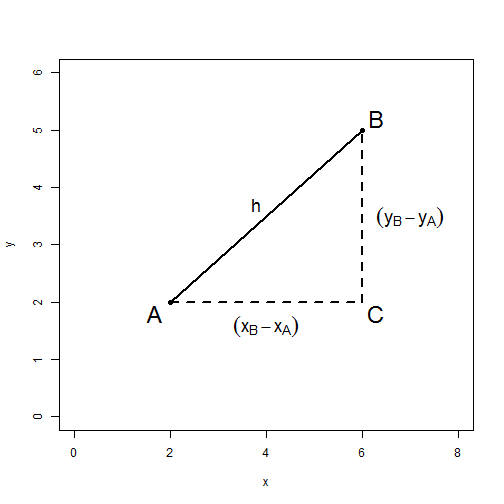
\includegraphics{figure/unnamed-chunk-10.png}
\caption{Figura 1}
\end{figure}

\textbf{Figura 1:} Los puntos A, B y C de coordenadas $(x_A, y_A)$,
$(x_B, y_B)$ y $(x_B, y_A)$ pueden formar un triángulo rectángulo como
muestra la figura, cuyos catetos tienen los valores indicados entre
paréntesis. Por lo tanto, la distancia entre A y B es la hipotenusa del
triángulo y se puede hallar con la fórmula de Pitágoras.\\Nota: puede
reproducir este gráfico con la función \texttt{plotTriang} contenida en
el script ``plotTriang.R''; además lo invitamos a que examine dicho
código si le interesa entender cómo se crea tal figura.

\begin{center}\rule{3in}{0.4pt}\end{center}

En el presente ejercicio vamos a utilizar este concepto, así como las
recién aprendidas funciones \texttt{which} y \texttt{which.max}, y
también \texttt{which.min}. La idea es encontrar distancias entre puntos
y determinar distancias mínimas y máximas. En el archivo ``dist.R'' el
código inicial (8 líneas) debería reproducir un gráfico muy similar a la
\textbf{Figura 2}.

\begin{figure}[htbp]
\centering
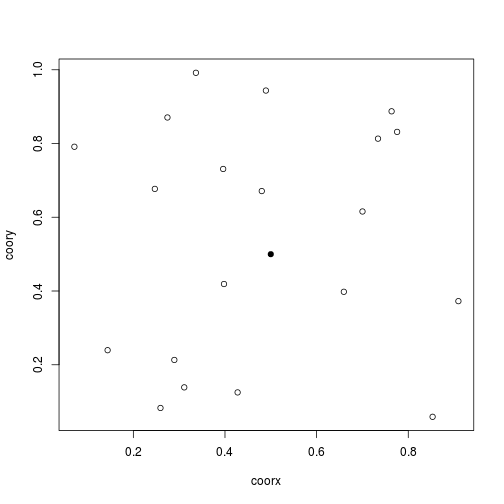
\includegraphics{figure/unnamed-chunk-11.png}
\caption{Figura 2}
\end{figure}

Los objetos \texttt{coorx} y \texttt{coory} son las coordenadas en los
ejes x e y respectivamente de todos los puntos blancos. Estos fueron
obtenidos con un generador de números aleatorios. El punto negro en el
centro de la figura es nuestro foco de interés.

Para encontrar cuáles son el más cercano y el más lejano del punto negro
primero debemos calcular las distancias desde éste a todos los demás.
Esto lo podemos hacer usando la función \texttt{hipot} creada
anteriormente. Para esto debemos calcular, con los valores de las
coordenadas, los ``catetos'', usando de referencia el método descripto
en la \textbf{Figura 1}. Para esto usted necesita saber que las
coordenadas del punto central son (0.5, 0.5).

Para comprobar que su resultado es correcto, puede utilizar el siguiente
código:

\begin{Shaded}
\begin{Highlighting}[]
\KeywordTok{plot}\NormalTok{(coorx, coory)}
\KeywordTok{points}\NormalTok{(}\FloatTok{0.5}\NormalTok{, }\FloatTok{0.5}\NormalTok{, }\DataTypeTok{pch =} \DecValTok{19}\NormalTok{)}
\KeywordTok{points}\NormalTok{(coorx[i], coory[i], }\DataTypeTok{pch =} \DecValTok{19}\NormalTok{, }\DataTypeTok{col =} \StringTok{"red"}\NormalTok{)}
\KeywordTok{points}\NormalTok{(coorx[j], coory[j], }\DataTypeTok{pch =} \DecValTok{19}\NormalTok{, }\DataTypeTok{col =} \StringTok{"darkgreen"}\NormalTok{)}
\end{Highlighting}
\end{Shaded}
Complete el código del archivo ``dist.R'' para completar esta parte del
ejercicio.

\subsection{2. Cálculo de sumatorias}

Crear el código necesario para calcular sumatorias en R u otros
lenguajes no es intiutivo cuando no se tiene experiencia en
programación. En R la función \texttt{sum} sirve para este propósito. Si
tenemos un vector \texttt{s} con una cantidad arbitraria de elementos,
entonces la suma de todos ellos se realiza con el comando
\texttt{sum(s)}. Por ejemplo:

\begin{Shaded}
\begin{Highlighting}[]
\NormalTok{s <- }\KeywordTok{c}\NormalTok{(-}\DecValTok{10}\NormalTok{, }\DecValTok{5}\NormalTok{, }\DecValTok{6}\NormalTok{)}
\KeywordTok{sum}\NormalTok{(s)}
\end{Highlighting}
\end{Shaded}
\begin{verbatim}
## [1] 1
\end{verbatim}
Nota: la función \texttt{c} aquí es usada para crear \texttt{s}, un
vector que es simplemente la secuencia de los números -10, 5, 6. Dicha
función es una de las más usadas en R.

Sin duda que este es el caso más trivial. Cuando queremos trabajar con
algún caso más elaborado, es conveniente entonces separar el problema en
dos partes, (1) Crear el vector \texttt{s}, el cual contiene todos los
términos de la sumatoria y (2) ejecutar la función \texttt{sum}, y es
por eso que así lo hicimos en el ejemplo. Por supuesto que en la primer
etapa es en donde se hace casi todo el trabajo. Muchas veces nos
encontramos con sumatorias que están definidas con funciones
matemáticas. Un ejemplo es la fórmula para calcular la varianza no
sesgada de una muestra de \texttt{n} datos:

\[
  \sigma ^ 2 = \frac{1}{n - 1} \cdot \sum_{i=1}^{i=n} (x_i - \overline{x}) ^ 2 
\]

En donde $\overline{x}$ denota el valor promedio de la muestra de datos,
calculado como $\frac{1}{n} \cdot \sum_i x_i$. Llamaremos ``término de
la sumatoria'' a la función está incluida en la misma, es decir
$(x_i - \overline{x}) ^ 2$.

\subsubsection{2.a Cálculo de la varianza de una muestra}

Script: varianza.R

En el archivo ``varianza.R'' usted deberá escribir los pasos necesarios
para calcular la varianza del vector \texttt{x} que se muestra en el
archivo (siga las instrucciones incluidas en los comentarios). Para
confirmar que su resultado es correcto, puede ejecutar el comando
\texttt{var(x)}, el cual debería devolver el mismo valor que el objeto
\texttt{out}.

\subsubsection{2.b Paradoja de Zenón}

Script: zenon.R

Según la clásica
\href{https://es.wikipedia.org/wiki/Paradojas\_de\_Zen\%C3\%B3n\#La\_dicotom.C3.ADa}{paradoja
de la dicotomía de Zenón}(http://xkcd.com/1153/) es imposible caminar de
un punto A a un punto B, debido a que primero debemos movernos la mitad
del camino, posteriormente avanzar la mitad de la mitad del camino y así
ad infinitum, sin llegar jamás a B. Esto se traduce en avanzar primero
1/2 de camino, luego 1/4, luego 1/8, luego 1/16 y así sucesivamente.
Entonces, luego de $n$ pasos de este tipo se alcanza una fracción de
camino equivalente a:

\[
  Z_n = \sum_{i=1}^{i=n} \frac{1}{2 ^ i} \;=\;
  \frac{1}{2 ^ 1} + \frac{1}{2 ^ 2} + \frac{1}{2 ^ 3} + ... + \frac{1}{2 ^ n} \;=\;
  \frac{1}{2} + \frac{1}{4} + \frac{1}{8} + ... + \frac{1}{2 ^ n}
\]

(¡nótese que el primer valor de $i$ es 1 y no 0!)

Si es cierta la proposición de Zenón, entonces no importa que tan grande
sea $n$, esta sumatoria siempre será menor a 1, a pesar de que el límite
de la misma cuando $n \to \infty$ es 1. Podemos verificar numéricamente
esta afirmación usando R: si elegimos un valor $\varepsilon$
arbitrariamente pequeño, entonces podemos encontrar un $n$ tal que
$1 - Z_n < \varepsilon$.

En este ejercicio, usted deberá completar el código del archivo
``zenon.R'' según las instrucciones que se indican en el mismo. Para que
usted pueda tener una referencia, considere que si el código se hace
correctamente, la sumatoria entonces para $n = 3$ el valor \texttt{out}
debería ser 0.875.

Además usted debe probar distintos valores del entero \texttt{n}, con el
fin de encontrar aquel entero mínimo necesario para lograr un valor de
\texttt{out} tal que la diferencia entre \texttt{out} y 1 debe ser menor
a 0.000001 (i.e.: 1e-06). Puede comprobar que su resultado cumple con
esa premisa con el comando \texttt{1 - out \textless{} 1e-06}.

Nota: en este ejercicio, y \emph{a diferencia de la mayoría de los
casos} de este curso, la respuesta para el valor de \texttt{n} debe ser
un número entero (i.e.: 42), el cual usted deberá escribir en la línea
correspondiente del archivo ``zenon.R''.

Para visualizar la convergencia de la serie puede usar el comando:

\begin{Shaded}
\begin{Highlighting}[]
\KeywordTok{plot}\NormalTok{(}\KeywordTok{cumsum}\NormalTok{(s), }\DataTypeTok{type =} \StringTok{"o"}\NormalTok{, }\DataTypeTok{xlab =} \StringTok{"n"}\NormalTok{, }\DataTypeTok{ylab =} \KeywordTok{expression}\NormalTok{(Z[n]))}
\end{Highlighting}
\end{Shaded}
\subsubsection{2.c Extra: series geométricas}

Script: geom.R

(\emph{Este ejercicio es opcional, aunque puede sumar puntos en su
calificación final del repartido})

La serie $Z_n$ es un caso particular de serie geométrica. La fórmula
general de este tipo de series es:

\[
  S_n = \sum_{i=0}^{i=n} \frac{1}{z ^ i}
\]

(Nota: ahora el primer término corresponde a i=0, por lo que a toda
$S_n$ se le agrega un +1 en comparación con la misma sumatoria empezando
por i=1.)

Un resultado importante es que la serie converge a un valor determinado
(es decir, tiene un límite finito para $n \to \infty$) para todos los z
tales que $1 > \|z\|$ (1 mayor al valor absoluto de $z$). El objetivo de
este ejercicio es confirmar este resultado. Para esto debe completarse
el código del archivo \texttt{geom.R}, siguiendo las instrucciones que
allí se indican.

Nota: en este ejercicio utilice valores para \texttt{n} y \texttt{z} a
elección (siendo el primero entero y positivo).

Si el código es correcto, el resultado \texttt{out} debería ser idéntico
(o casi igual, debido a pequeños errores numéricos de redondeo) al valor
de la siguiente fórmula:

\[
  S_n = \frac{1 - z ^ {- n}}{1 - z ^ {-1}}
\]

\begin{center}\rule{3in}{0.4pt}\end{center}

\subsection{3. Índice de Shannon-Wiener}

El índice de
\href{https://es.wikipedia.org/wiki/\%C3\%8Dndice\_de\_Shannon}{Shannon-Wiener}
o simplemente índice de Shannon ha sido utilizado en ecología y otras
ciencias como indicador de diversidad de una comunidad de especies. Este
índice fue creado originalmente para ser usado como medida de entropía
en cadenas de caracteres (i.e., texto) en el contexto de la teoría de la
información (\href{http://www.amazon.com/dp/0444538682}{Legendre \&
Legendre, 2012}). En general para una colección de objetos de distintas
categorías (i.e., individuos de distintas especies), el índice de
Shannon se calcula con la siguiente fórmula:

\[
  H = - \sum_{i=1}^{i=S} p_i \cdot log_2 (p_i)
\]

(La base del logaritmo no es demasiado importante, pero en este
ejercicio nos vamos a regir a esta definición en particular; es decir,
vamos a usar logarítmo de base 2)

Aquí $S$ es el número total de categorías o especies y $p_i$ es la
frecuencia relativa de la categoría i. Es decir:

\[
  p_i = \frac{n_i}{N}
\]

En donde $n_i$ es la cantidad de objetos de la categoría $i$ contenidos
en nuestra colección y $N$ es la cantidad total de objetos. Por ejemplo,
para la palabra ``banana'', los $p_i$ de las letras ``a'', ``b'' y ``n''
son $3/6$, $1/6$ y $2/6$ respectivamente y el $H$ resultante es 1.46.

\subsubsection{3.a Cálculo de H para una colección de números}

Script: shannon-1.R

En el archivo ``shannon-1.R'' usted encontrará código de R incompleto.
El objetivo de este script es calcular el $H$ de un vector de números
llamado \texttt{coleccion}. Pero a diferencia del ejercicio 2, vamos a
utilizar otra estrategia para de hacer la sumatoria necesaria, a través
del operador \texttt{\%*\%} de R.

Una forma de hacer sumatorias del tipo $\sum v_i \cdot u_i$ es usando el
\href{https://es.wikipedia.org/wiki/Producto\_escalar}{producto escalar}
o producto interior de vectores, para lo cual en R se usa el operador
\texttt{\%*\%}. Específicamente, si $v$ y $u$ son vectores columna,
entonces $\langle v, u \rangle = \sum v_i \cdot u_i$. Otra
representación común es:

\[
  v^T \cdot u = (v_1 v_2 \cdots v_d)
    \begin{pmatrix}
      u_1 \\
      u_2 \\
      \vdots \\
      u_d
    \end{pmatrix}
\]

en dónde $v^T$ es el vector columna $v$ transpuesto y $d$ es la
dimensión o número de elementos de ambos vectores. En R el producto
escalar se escribe

\begin{Shaded}
\begin{Highlighting}[]
\NormalTok{v %*% u}
\end{Highlighting}
\end{Shaded}
simplemente, ignorando detalles de transposición. De hecho los vectores
en R no son fila o columna, si no que simplemente son una secuencia de
elementos. En general este operador sirve para toda multiplicación de
matrices en R.

En este ejercicio deberá completar el archivo ``shannon-1.R'' de forma
que sea capaz de calcular el valor de H para el vector
\texttt{coleccion} o \emph{cualquier otro vector} de R, utilizando el
producto escalar de vectores para calcular el resultado de la sumatoria.
Para el caso particular de \texttt{coleccion}, el $H$ esperado es de
2.699514.

\paragraph{Observaciones a tener en cuenta:}

El cálculo del $H$ puede dividirse en (1) calcular los valores de $p_i$
y (2) realizar la sumatoria. Para calcular los $p_i$ es necesario a su
vez tener los $n_i$ y el valor $N$. Para estas tareas las funciones
\texttt{table} y \texttt{length} pueden ser de gran ayuda. La primera
sirve para hacer un conteo de la cantidad de objetos por categoría,
mientras que la función \texttt{length} devuelve la cantidad de
elementos de un vector cualquiera. No dude en consultar la documentación
de R de estas dos funciones en caso de que no comprenda del todo bien su
accionar.

\subsubsection{3.b Extra: función \texttt{shannon}}

Script: shannon-2.R

(\emph{Este ejercicio es opcional, aunque puede sumar puntos en su
calificación final del repartido})

El archivo ``shannon-2.R'' contiene el código incompleto necesario para
crear una función que calcule el índice de Shannon para cualquier vector
de R. Si le resulta útil, utilice la función \texttt{prp} creada en la
lección 1.2 (``una sesión de ejemplo'') como referencia.

Tenga en cuenta que en los paréntesis vacíos de luego de
\texttt{function} es en donde se ponen los argumentos o entradas de la
función. Esta función sólo debería usar un argumento; el nombre elegido
el mismo debe ser mismo que se use luego en los comandos internos de la
misma (los comandos comprendidos entre las llaves \texttt{\{\}}).

Si su función está correcta, el siguiente código debería correr
correctamente y el resultado debería ser el predicho por el objeto
\texttt{frase}:

\begin{Shaded}
\begin{Highlighting}[]
\NormalTok{frase <- }\StringTok{"Esta frase tiene un H = 3.7"}
\NormalTok{x <- }\KeywordTok{strsplit}\NormalTok{(frase, }\StringTok{""}\NormalTok{)[[}\DecValTok{1}\NormalTok{]]}
\KeywordTok{shannon}\NormalTok{(x)}
\end{Highlighting}
\end{Shaded}
\begin{verbatim}
## [1] 3.708
\end{verbatim}
(Nota: el segundo comando toma la \texttt{frase} y la parte en todos los
caracteres que la componen)

\end{document}
